%!TEX root = notes.tex

\chapter{Numerical Approximation for Unconstrained Optimization}\label{chapter:nonlinearoptimization}
Although technically any characterization result finds the exact value of the extrema of a function, computationally this is hardly feasible (specially for functions of very high dimension).  See the following session based on problem \ref{problem:tricky} for an example, where we try to find the critical points of the function $f(x,y,z)=e^{x^2+y^2+z^2}-x^4-y^y-z^6$ symbolically in Python with the \texttt{sympy} libraries:

% framesep=2mm,
% baselinestretch=1.2,
\begin{minted}[frame=single, fontsize=\footnotesize, linenos ]{python}
# Importing necessary symbols/libraries/functions
from sympy.abc import x,y,z
from sympy import Matrix, solve, exp
from sympy.tensor.array import derive_by_array

# Description of f, computation of its gradient and Hessian
f = exp(x**2 + y**2 + z**2) - x**4 -y**6 - z**6
gradient = derive_by_array(f, [x,y,z])
hessian  = Matrix([derive_by_array(gradient, a) for a in [x,y,z]])
\end{minted}
While the correct expressions for $\gradient{f}$ and $\Hess{f}$ are quickly computed, trying to find critical points results in an error:
\begin{minted}[frame=single,fontsize=\footnotesize, linenos, firstnumber=10,mathescape]{python}
# Search of critical points by solving $\gradient{f}=0$
solve(gradient)
\end{minted}

\begin{minted}[frame=lines,fontsize=\footnotesize]{python}
NotImplementedError: could not solve 
4*x**2*sqrt(-log(exp(x**2)/(2*x**2))) - 6*(-log(exp(x**2)/(2*x**2)))**(5/2)
\end{minted}

Too complex a task to be performed symbolically, although the obvious answer is $(0,0,0)$.  A better way to approach this is by trying to approximate this minimum using the structure of the graph of $f$.  In these notes we are going to explore several strategies to accomplish this task, based on the concept of \emph{iterative methods for finding zeros of real-valued functions}.

\begin{example}[The Newton-Raphson method]
In order to find a many correct decimal places of $\sqrt{2}$, we allow a computer to find better and better approximations of the solution of the equation $f(x)=x^2-2$.  We start with a decent guess, say $x_0=3$.  We construct a sequence $\{ x_n \}_{n\in\field{N}}$ that converges to $\sqrt{2}$ as follows:
\begin{enumerate}
\item Find the tangent line to the graph of $f$ at $x_0$, 
\begin{equation*}
y-f(x_0)=f'(x_0)(x-x_0)
\end{equation*}
\item Provided this line is not horizontal ($f'(x_0)\neq 0$), report the intersection of this line with the $x$--axis.  Call this intersection $x_1$
\begin{equation*}
x_1=x_0-\frac{f(x_0)}{f'(x_0)}
\end{equation*}
\item Repeat this process, to get the sequence 
\begin{equation*}
x_{n+1} = x_n- \frac{f(x_n)}{f'(x_n)}
\end{equation*}
\end{enumerate}
\begin{figure}[ht!]
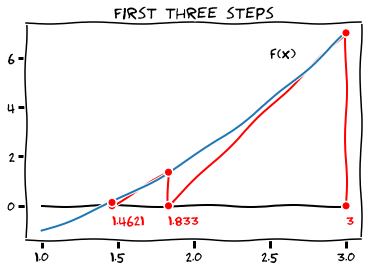
\includegraphics[width=0.65\linewidth]{newton1.png}
\caption{Newton-Raphson iterative method}
\label{figure:Newton-Raphson}
\end{figure}
Note the result of applying this process a few times:

\begin{table}[ht!]
\begin{tabular}{|c|c|r|} \hline 
$n$ & $x_n$ & $f(x_n)$ \\ \hline \hline 
$0$ & $3.000000000000000$ & $7.0000E+00$ \\ \hline 
$1$ & $1.833333333333333$ & $1.3611E+00$ \\ \hline 
$2$ & $1.462121212121212$ & $1.3780E-01$ \\ \hline 
$3$ & $1.414998429894803$ & $2.2206E-03$ \\ \hline 
$4$ & $1.414213780047198$ & $6.1568E-07$ \\ \hline 
$5$ & $1.414213562373112$ & $4.7518E-14$ \\ \hline 
$6$ & $1.414213562373095$ & $-4.4409E-16$ \\ \hline 
$7$ & $1.414213562373095$ & $4.4409E-16$ \\ \hline 
\end{tabular}
\caption{Convergence to $\sqrt{2}$ with 15-digit accuracy in 6 steps}
\label{table:Newton-Raphson}
\end{table}
\end{example}

Let's proceed to extend this process to functions $\boldsymbol{g} \colon \field{R}^d \to \field{R}^d$ as follows.  
\begin{itemize}
	\item Any function $\boldsymbol{g} \colon \field{R}^d \to \field{R}^d$ can be described in the form $\boldsymbol{g}(\x) = \big( g_1(\x), g_2(\x), \dotsc, g_d(\x) \big)$ for $d$ real-valued functions $g_k\colon \field{R}^d \to \field{R}$ ($1\leq k \leq d$).
	\item For such a function $\boldsymbol{g}$, we may express its gradient as a $d\times d$ matrix in the form
	\begin{equation*}
	\gradient{\boldsymbol{g}} = \begin{bmatrix}
	\frac{\partial g_1}{\partial x_1} & \frac{\partial g_1}{\partial x_2} & \dotsb & \frac{\partial g_1}{\partial x_d} \\ \\
	\frac{\partial g_2}{\partial x_1} & \frac{\partial g_2}{\partial x_2} & \dotsb & \frac{\partial g_2}{\partial x_d} \\ \\
	\vdots & \vdots & \ddots & \vdots \\ \\
	\frac{\partial g_d}{\partial x_1} & \frac{\partial g_d}{\partial x_2} & \dotsb & \frac{\partial g_d}{\partial x_d} \\
	\end{bmatrix}
	\end{equation*}
\end{itemize}
Start with a guess for the solution, $\x_0$, and on the $n$--th step of the algorithm compute the $(n+1)$--th term of the sequence by
\begin{equation*}
\x_{n+1} = \x_n - \big[ \gradient{\boldsymbol{g}}(\x_n) \big]^{-1} \boldsymbol{g}(\x_n),
\end{equation*}
where $\big[ \gradient{\boldsymbol{g}}(\x_n) \big]^{-1}$ represents the inverse matrix of the gradient at $\x_n$.  This is equivalent to selecting in the tangent hyperplane to the graph of $\boldsymbol{g}$ at $\boldsymbol{g}(\x_n)$, the one line in the direction with the most rapid increase/decrease.  The computation of $\x_{n+1}$ is therefore the intersection of that line with the hyperplane $x_d=0$.

\begin{example}\label{example:preNewton4poly4}
Consider the function $\boldsymbol{g}\colon \field{R}^2 \to \field{R}^2$ given by
\begin{equation*}
\boldsymbol{g}(x,y,z) = \big( x^3-y, y^3-x \big)
\end{equation*}
Its gradient at each $(x,y)$ is given by
\begin{equation*}
\gradient{\boldsymbol{g}}(x,y) = \begin{bmatrix} 3x^2 & -1 \\ -1 & 3y^2 \end{bmatrix}
\end{equation*}
Note the determinant of this matrix is $\det \gradient{\boldsymbol{g}}(x,y) = 9x^2y^2-1 = (3xy-1)(3xy+1)$.  For any point $(x,y)$ that does not make this expression zero, this is an invertible matrix with 
\begin{equation*}
\big[ \gradient{\boldsymbol{g}}(x,y)\big]^{-1} = \frac{1}{9x^2y^2-1}\begin{bmatrix} 3y^2 & 1 \\ 1 & 3x^2 \end{bmatrix}
\end{equation*}
For a decent guess $(x_0, y_0)$, the sequence computed by the Newton method is then given by
\begin{align*}
\begin{bmatrix} x_{n+1} \\ y_{n+1} \end{bmatrix} &= \begin{bmatrix} x_n \\ y_n \end{bmatrix} -\frac{1}{9 x_n^2 y_n^2-1}\begin{bmatrix} 3y_n^2 & 1 \\ 1 & 3x_n^2 \end{bmatrix} \begin{bmatrix} x_n^3-y_n \\ y_n^3-x_n \end{bmatrix} \\
&= \begin{bmatrix}
x_n - \frac{3x_n^3 y_n^2-2 y_n^3-x_n}{9x_n^2  y_n^2-1} \\  y_n - \frac{3x_n^2 y_n^3+-2x_n^3- y_n}{9x_n^2 y_n^2-1}
\end{bmatrix}
\end{align*}
Let's run this process with three different initial guesses:
\begin{enumerate}
	\item Starting at $(x_0, y_0) = (-1.0,1.0)$, the sequence converges to $(0,0)$.  %See Table \ref{table:00}.
	\begin{table}[ht!]
	\begin{tabular}{|c|c|c|} \hline 
	$n$ & $x_n$ & $y_n$ \\ \hline \hline 
	$0$ & $-1.00000000$ & $1.00000000$ \\ \hline 
	$1$ & $-0.50000000$ & $0.50000000$ \\ \hline 
	$2$ & $-0.14285714$ & $0.14285714$ \\ \hline 
	$3$ & $-0.00549451$ & $0.00549451$ \\ \hline 
	$4$ & $-0.00000033$ & $0.00000033$ \\ \hline 
	$5$ & $-0.00000000$ & $0.00000000$ \\ \hline 
	$6$ & $-0.00000000$ & $0.00000000$ \\ \hline 
	\end{tabular}
	\caption{Convergence to $(0,0)$ in 5 steps}
	\label{table:00}
	\end{table}
	\item Starting at $(x_0,y_0) = (3.5, 2.1)$, the sequence converges to $(1,1)$.  %See Table \ref{table:11}.
	\begin{table}[ht!]
	\begin{tabular}{|c|c|c|} \hline 
	$n$ & $x_n$ & $y_n$ \\ \hline \hline 
	$0$ & $3.50000000$ & $2.10000000$ \\ \hline 
	$1$ & $2.37631607$ & $1.57961573$ \\ \hline 
	$2$ & $1.65945969$ & $1.27476534$ \\ \hline 
	$3$ & $1.23996276$ & $1.10419072$ \\ \hline 
	$4$ & $1.04837462$ & $1.02274752$ \\ \hline 
	$5$ & $1.00260153$ & $1.00133122$ \\ \hline 
	$6$ & $1.00000824$ & $1.00000451$ \\ \hline 
	$7$ & $1.00000000$ & $1.00000000$ \\ \hline 
	$8$ & $1.00000000$ & $1.00000000$ \\ \hline 
	\end{tabular}
	\caption{Convergence to $(1,1)$ in 7 steps}
	\label{table:11}
	\end{table}
	\item Starting at $(x_0, y_0) = (-13.5, -7.3)$, the sequence converges to $(-1,-1)$.  %See Table \ref{table:-1-1}.
	\begin{table}[ht!]
	\begin{tabular}{|c|c|c|} \hline 
	$n$ & $x_n$ & $y_n$ \\ \hline \hline 
	$0$ & $-13.50000000$ & $-7.30000000$ \\ \hline 
	$1$ & $-9.00900415$ & $-4.92301873$ \\ \hline 
	$2$ & $-6.01982204$ & $-3.36480659$ \\ \hline 
	$3$ & $-4.03494126$ & $-2.36199873$ \\ \hline 
	$4$ & $-2.72553474$ & $-1.73750959$ \\ \hline 
	$5$ & $-1.87830623$ & $-1.36573112$ \\ \hline 
	$6$ & $-1.36121191$ & $-1.15374930$ \\ \hline 
	\end{tabular}
	\begin{tabular}{|c|c|c|} \hline 
	$n$ & $x_n$ & $y_n$ \\ \hline \hline 
	$7$ & $-1.09518303$ & $-1.04341362$ \\ \hline 
	$8$ & $-1.00932090$ & $-1.00463507$ \\ \hline 
	$9$ & $-1.00010404$ & $-1.00005571$ \\ \hline 
	$10$ & $-1.00000001$ & $-1.00000001$ \\ \hline 
	$11$ & $-1.00000000$ & $-1.00000000$ \\ \hline 
	$12$ & $-1.00000000$ & $-1.00000000$ \\ \hline 
	$13$ & $-1.00000000$ & $-1.00000000$ \\ \hline 
	\end{tabular}
	\caption{Convergence to $(-1,-1)$ in 11 steps}
	\label{table:-1-1}
	\end{table}
\end{enumerate}
\end{example}

We can readily see how this process aids in the computation of critical points of a real-valued function $f\colon \field{R}^d \to \field{R}$:
\begin{enumerate}
	\item Set $\boldsymbol{g}(\x) = \gradient{f}(\x) = \big[ \frac{\partial f}{\partial x_1}, \dotsc, \frac{\partial f}{\partial x_d} \big]$
	\item It is then $\gradient{\boldsymbol{g}}(\x) = \Hess{f}(\x)$
	\item Perform a Newton method with a decent initial guess $\x_0$ on $\boldsymbol{g}=\gradient{f}$ to obtain the sequence
	\begin{equation*}
	\x_{n+1} = \x_n - \big[ \Hess{f}(\x_n) \big]^{-1} \cdot \gradient{f}(\x_n)
	\end{equation*}
\end{enumerate}

\begin{example}
Consider the function $f(x,y) = x^4-4xy+y^4$ over $\field{R}^2$.  Notice $\gradient{f}(x,y) = \big( x^3-y, y^3-x \big)$, as function $\boldsymbol{g}$ in Example \ref{example:preNewton4poly4}.  The critical points we found were $(0,0)$, $(-1,-1)$ and $(1,1)$.
\end{example}
\begin{example}
A similar process for the Rosenbrock function $\mathcal{R}_{1,1}(x,y) = (1-x)^2 + (y-x^2)^2$ gives the following recurrence formula:
\begin{align*}
\begin{bmatrix} x_{n+1} \\ y_{n+1} \end{bmatrix} &=
\begin{bmatrix} x_{n} \\ y_{n} \end{bmatrix} - \big[ \Hess{\mathcal{R}_{1,1}}(x_n,y_n) \big]^{-1} \cdot \gradient{\mathcal{R}_{1,1}}(x_n, y_n) \\
&= \begin{bmatrix} x_{n} \\ y_{n} \end{bmatrix} - \frac{2}{2x^2-2y+1} \begin{bmatrix}
1/2 & x \\ x & 6x^2-2y+1
\end{bmatrix} \begin{bmatrix}
2x^3-2xy+x-1 \\ y-x^2
\end{bmatrix} \\
&= \frac{1}{2x^2-2y+1} \begin{bmatrix}
2x^3-2xy+1 \\ x(2x^3-2xy-x+2)
\end{bmatrix}
\end{align*}
Starting with initial guess $(x_0, y_0) = (-2,2)$, the sequence converges to the critical point $(1,1)$.  
\end{example}
\begin{figure}[ht!]
\begin{tabular}{cc}
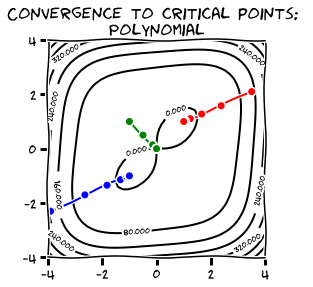
\includegraphics[width=0.45\linewidth]{convergenceNewton.png} &
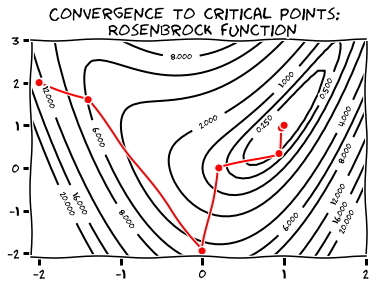
\includegraphics[width=0.55\linewidth]{convergenceNewtonRosenbrock.png} 
\end{tabular}
\caption{Newton method}
\label{figure:NewtonConvergence}
\end{figure}
